\section*{Log ud}
Log ud inddeles i en boundary og en dertilhørende controller, som det fremgår af \autoref{fig:MVCLogUd}. 

\begin{figure} [H]
\centering
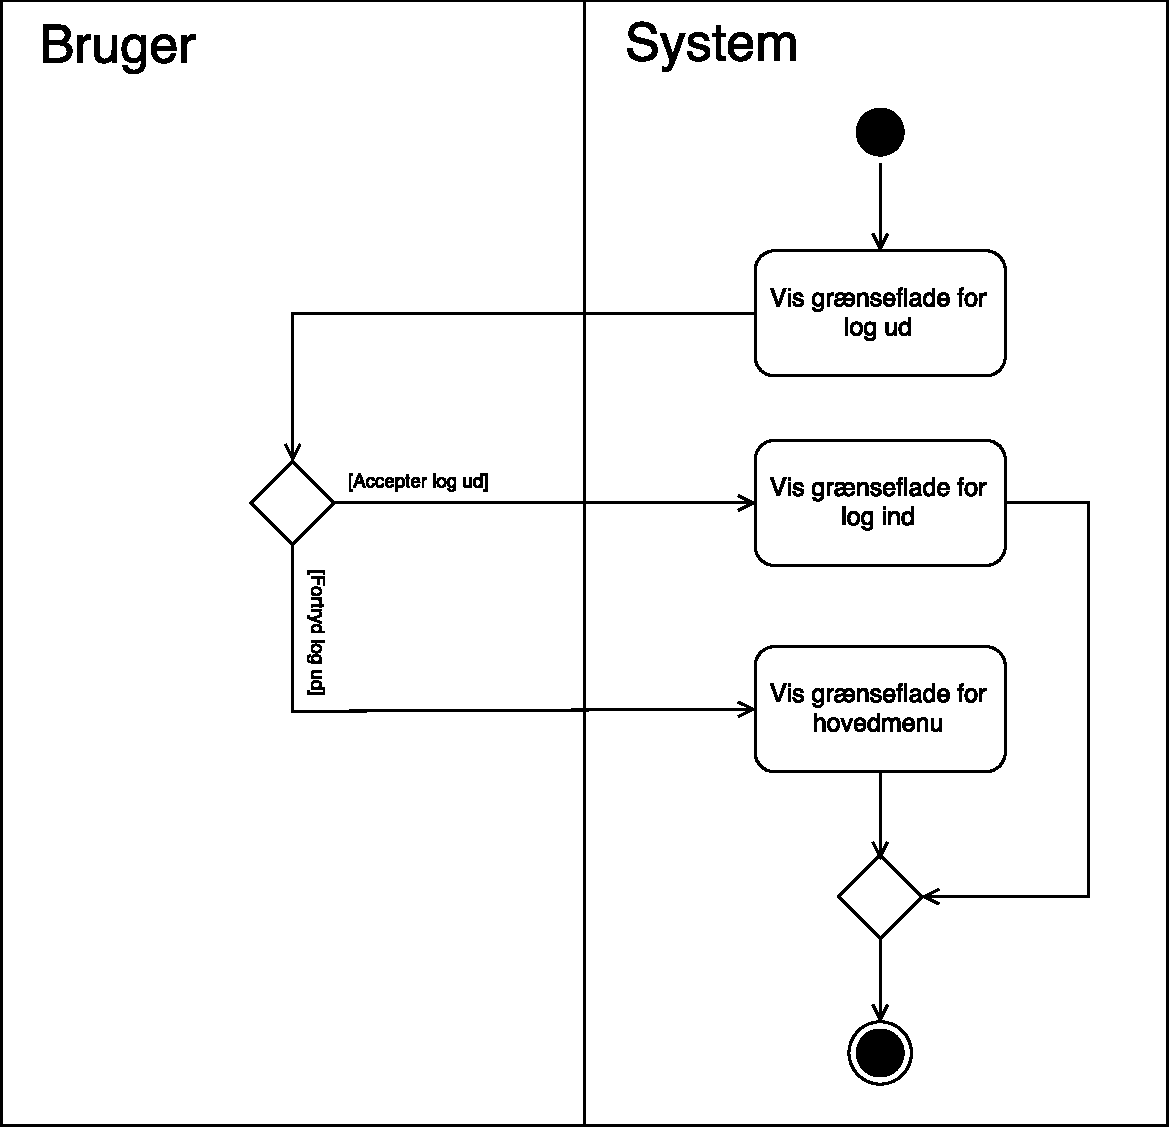
\includegraphics[width=0.6\textwidth]{figures/MVC/Logud}
\caption{Designklasser for log ud. Til venstre ses boundary og til højre controller.}
\label{fig:MVCLogUd}
\end{figure}

\noindent
Der opstilles i log ud et tekstfelt, af typen TextView, for log ud. Dertil opstilles en OKKnap og FortrydKnap af typen Button. 
Den tilhørende controller indeholder metoderne, Lyt, Vis, Nulstil, Send, Gem og Start. I sammenspil med designklasserne er der opstillet et sekvensdiagram, som fremgår af \autoref{fig:SEKlogUd}.

\begin{figure} [H]
\centering
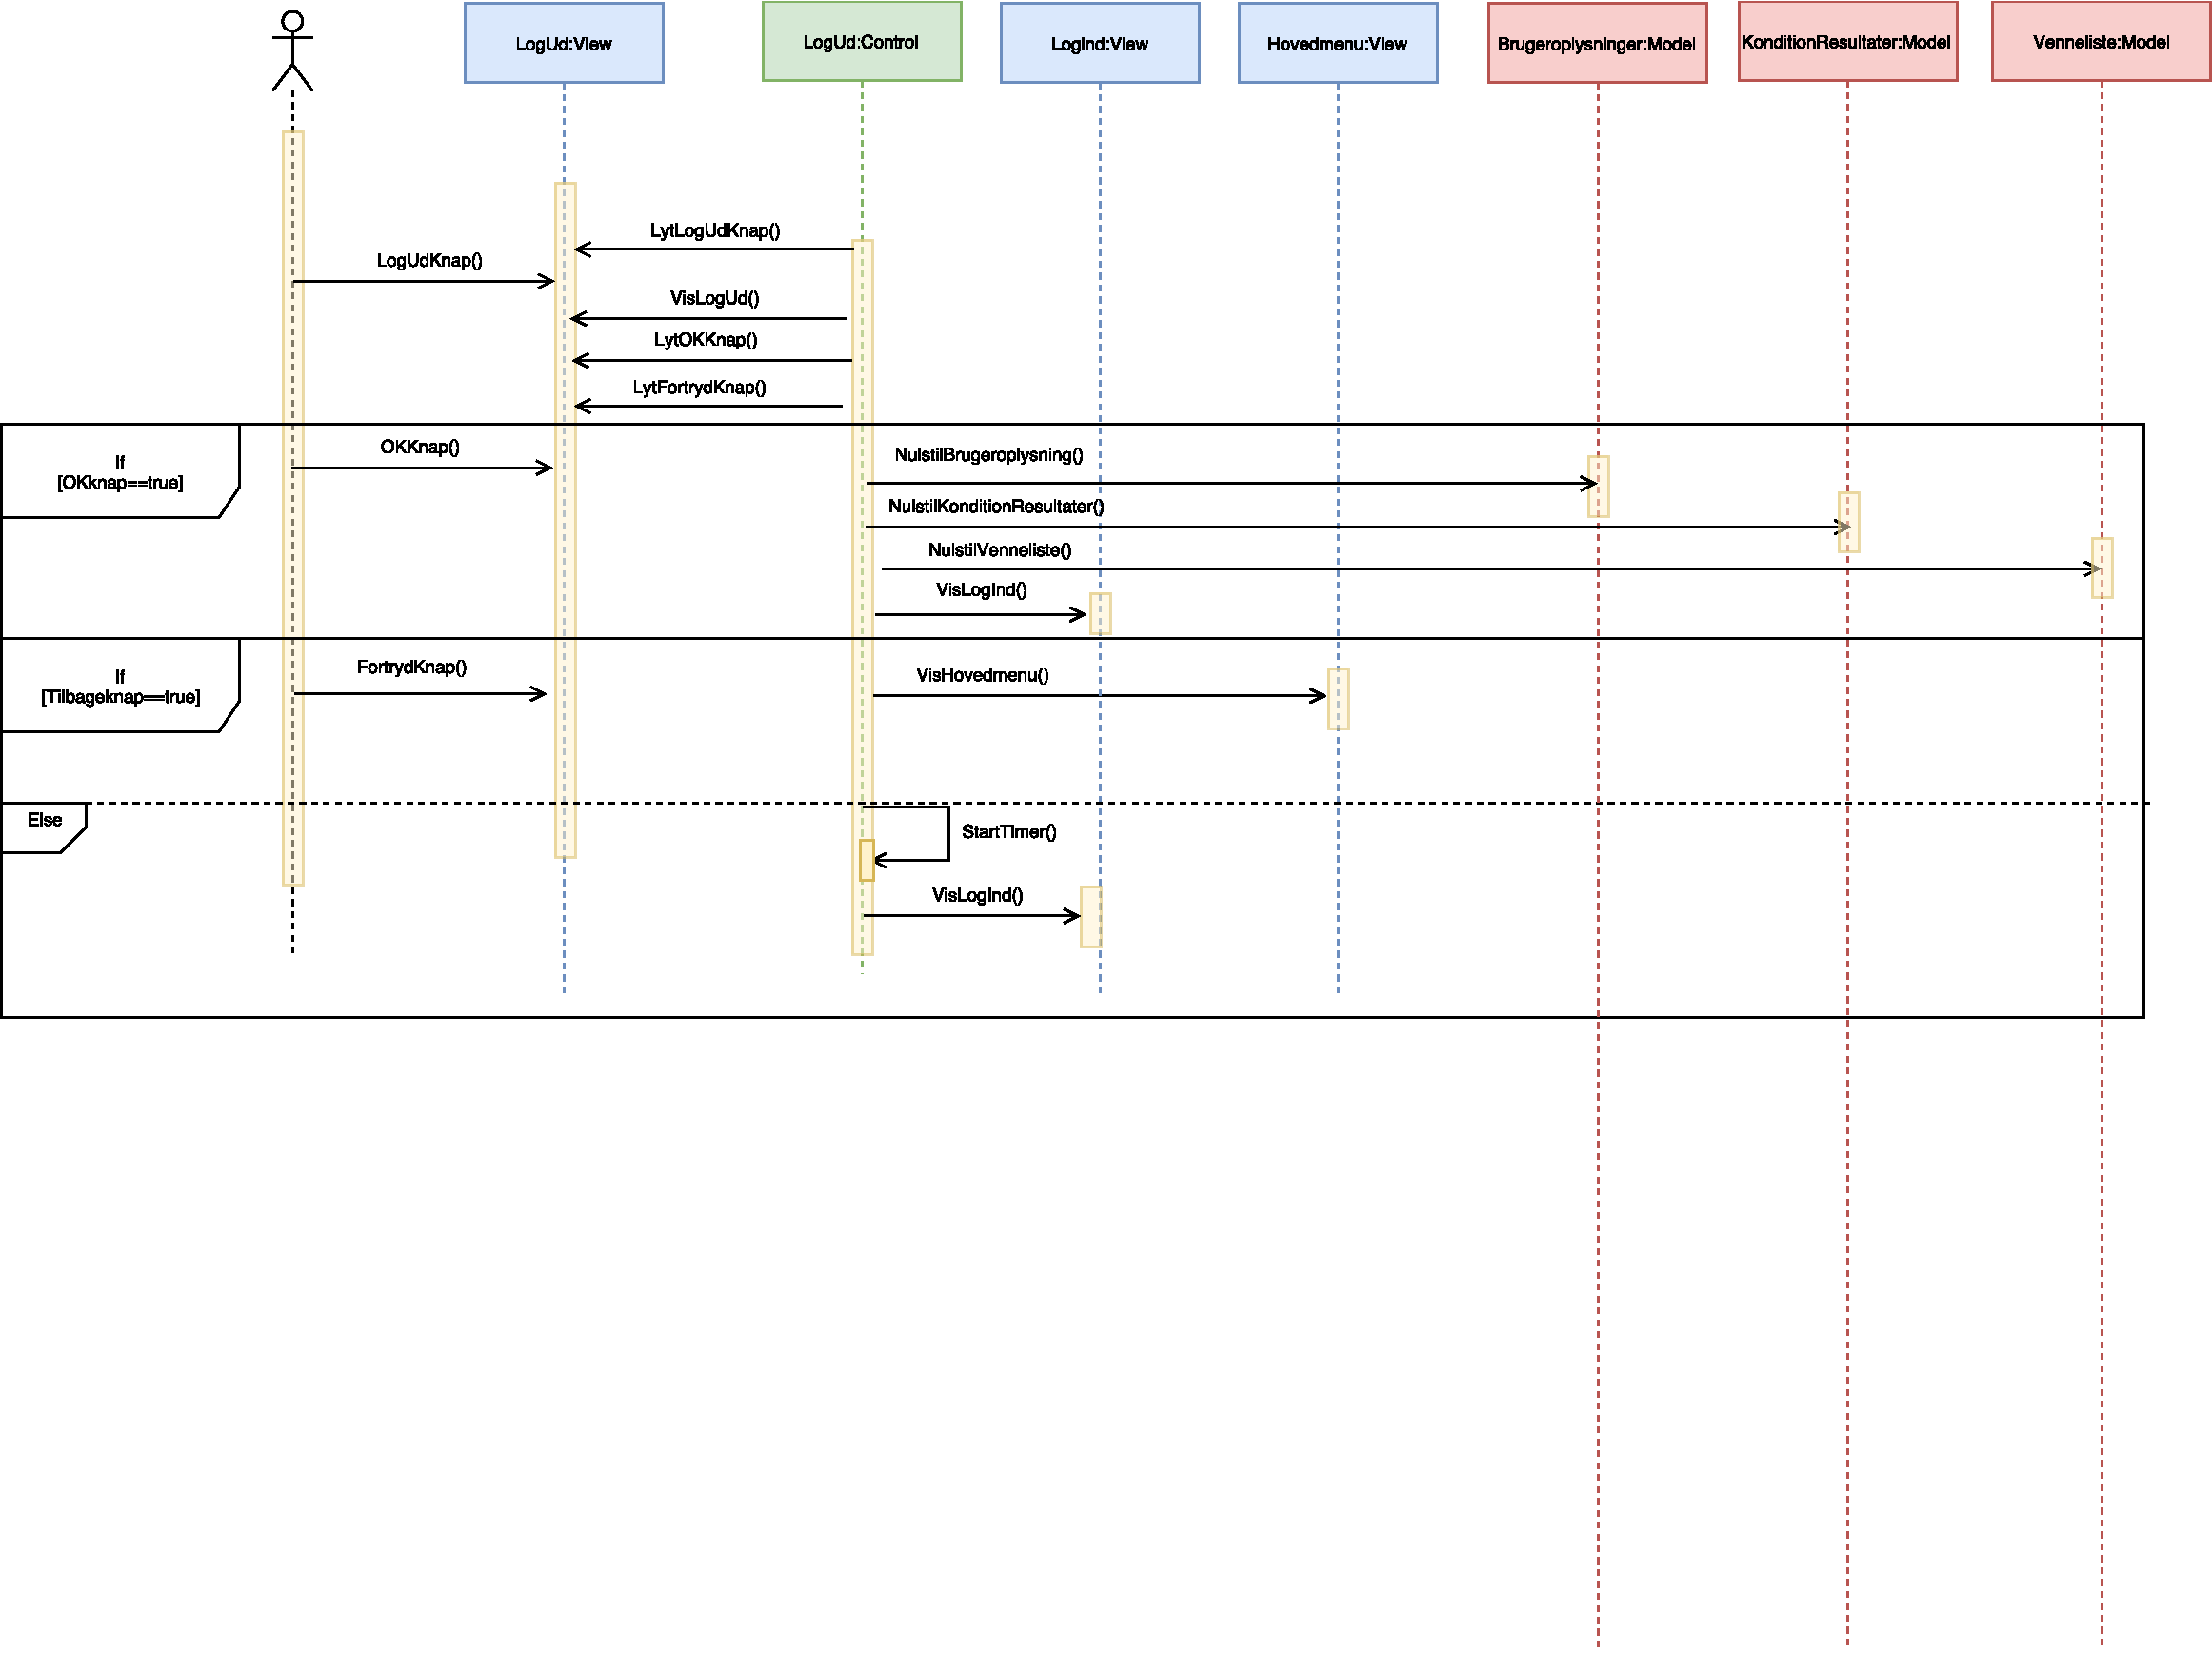
\includegraphics[width=1.55\textwidth, angle=90]{figures/Sek/SEKLogUd}
\caption{Sekvensdiagram for log ud.}
\label{fig:SEKlogUd}
\end{figure}

\noindent
Når brugeren via grænsefladen for hovedmenuen trykker på knappen for log ud vises grænsefladen for \textit{Log ud}. Her har brugeren mulighed for at trykke på OKKnap eller FortrydKnap. Hvis brugeren trykker på OKKnap eller timer udløst nulstiller controlleren, \textit{Log ud}, modellen for Brugeroplysninger. Herefter sendes besked til modellerne KonditionResultater og Venneliste om at gemme oplysningerne i databasen, hvorefter modellerne nulstilles. Grænsefladen for \textit{Log ind} vises efterfølgende, så brugeren har mulighed for at logge ind igen. Trykker brugeren på FortrydKnap, vises grænsefladen for hovedmenu igen. Hvis brugeren ikke angiver noget vil den forblive på grænsefladen for \textit{Log ud}. 
